\section{Verification of the Model}

To verify the model in simulation \eqref{FrameEq4TaylerApprox} is transformed into the Laplace domain, after which a transfer function of the system is derived. The proceeding equations are valid only around the operating point, and so for better overview, in the following \si{\Delta \theta_F = \theta_F}.
%
\begin{flalign}
	\eq{(J_F+m_w \cdot {l_w}^{2}) \cdot \theta_F \cdot s^2}{-B_F \theta_F\cdot s +  ( m_F \cdot l_F + m_w \cdot l_w ) g \cdot \theta_F - \tau_m + B_w \theta_w\cdot s } \unit{N \cdot m}
\label{LaplaceOfLinearizedModel}
\end{flalign}
%
The angle of the reaction wheel, \si{\theta_w}, still features in \eqref{LaplaceOfLinearizedModel}. It is desireable to have only one input, \si{\tau_m}, and one output, \si{\theta_F}. To achieve this, \eqref{WheelRotEq2} is transformed into the Laplace domain and solved for \si{\theta_w}.
%
\begin{flalign}
	\eq{\theta_w\cdot s^2} {\frac{\tau_m - B_w \theta_w\cdot s}{J_w} - \theta_F\cdot s^2}   &\\
	\eq{\theta_w} {\frac{ -J_w \theta_F \cdot s^2 + \tau_m }{ J_w \cdot s^2 + B_w \cdot s }}&
\label{WheelRotEq2Laplace}
\end{flalign}
%
\Eqref{WheelRotEq2Laplace} is now substituted for \si{\theta_w} in \eqref{LaplaceOfLinearizedModel}, and the transfer function is of the system is derived.
%
\begin{flalign}
	\eqOne{(J_F+m_w \cdot {l_w}^{2}) \cdot \theta_F \cdot s^2}{-B_F \theta_F\cdot s +  ( m_F \cdot l_F + m_w \cdot l_w ) g \cdot \theta_F - \tau_m}
	\eqTwo{+ B_w ( \frac{ -J_w \theta_F \cdot s^2 + \tau_m }{ J_w \cdot s^2 + B_w \cdot s } )\cdot s }&\nonumber
\label{CubliTransferFunction}
\end{flalign}
\vspace{-.2cm}
\large{\si{\frac{\theta_F}{\tau_m} =}}\nolinebreak
\Large{
\si{\frac{\frac{s}{-J_F - m_w \cdot {l_w}^2}}{s^3 + \left( \frac{B_w}{J_w} + \frac{B_w + B_F}{J_F + m_w \cdot {l_w}^2} \right) s^2 - \left( \frac{ \left( m_F \cdot l_F + m_w \cdot l_w \right)\cdot g}{ \left( J_F + m_w \cdot {l_w}^2 \right) J_w} - \frac{B_F B_w}{ \left(J_F + m_w \cdot {l_w}^2 \right) J_w} \right) s - \frac{\left(m_F \cdot l_F + m_w \cdot l_w \right) B_w\cdot g}{\left(J_F + m_w \cdot {l_w}^2 \right) J_w} }}}\normalsize\vspace{-1.9cm}\\
\vspace{1.8cm}\begin{flalign}\label{2ndCubliTransferFunction}\end{flalign}

\begin{figure}[H] 
	\centering 
	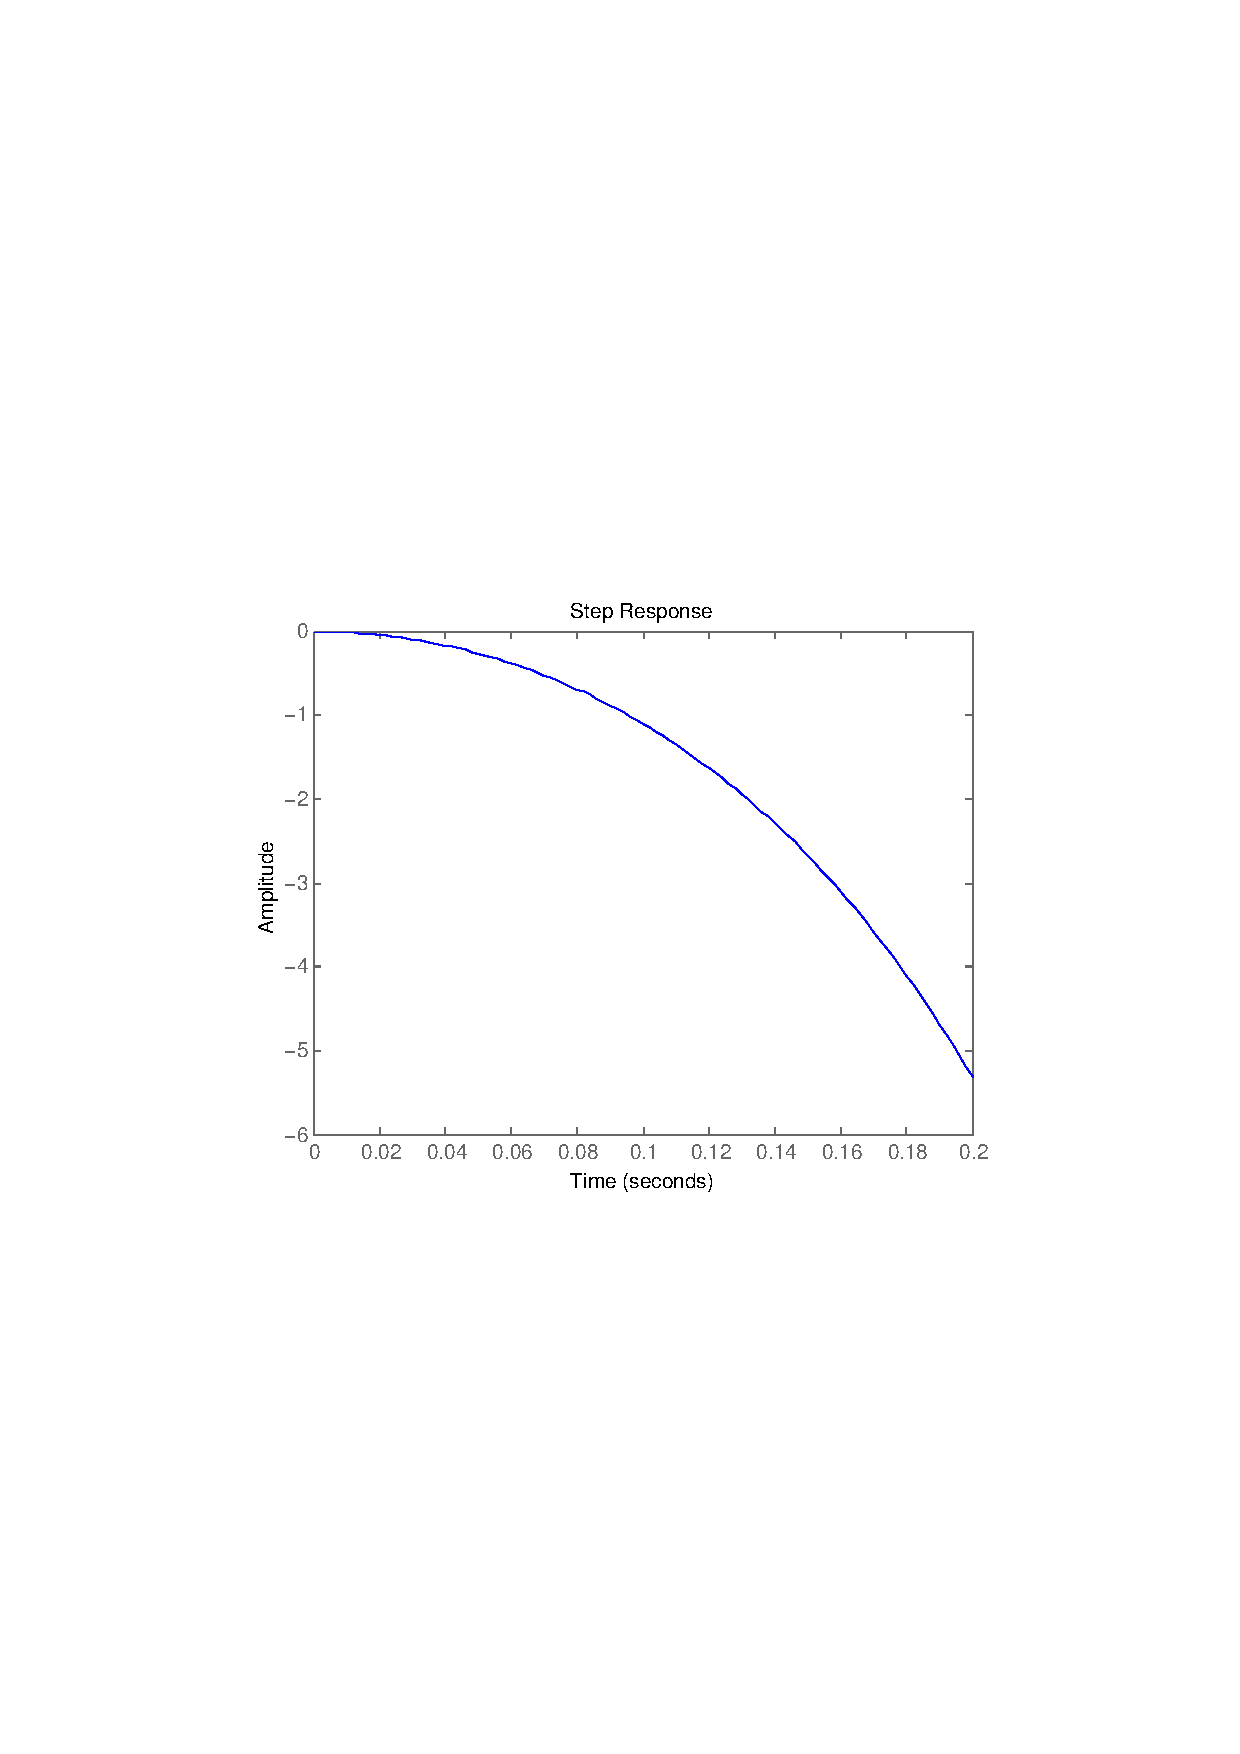
\includegraphics[scale=0.8]{figures/stepResponseTF}
	\centering
	\captionsetup{justification=centering}	
	\caption{Step response of the transfer function of the Cubli, G(s)}
	\label{stepCubliTF}
\end{figure}


\begin{figure}[H] 
	\centering 
	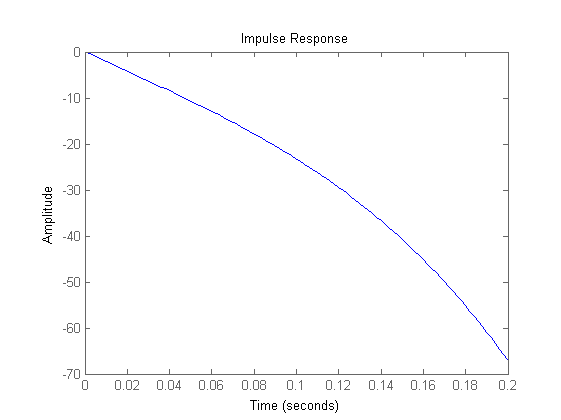
\includegraphics[scale=0.8]{figures/impulseResponseTF}
	\centering
	\captionsetup{justification=centering}	
	\caption{Impulse response of G(s)}
	\label{impulseCubliTF}
\end{figure}

\begin{figure}[H] 
	\centering 
	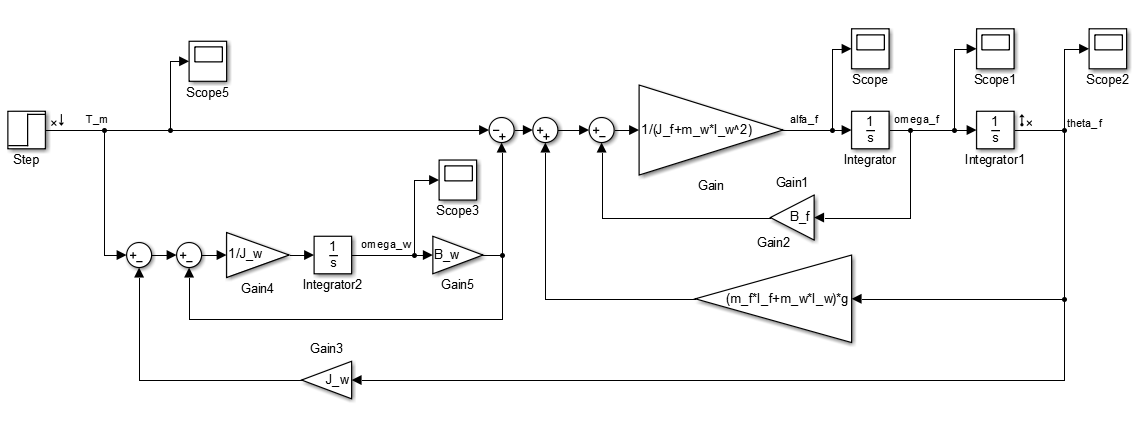
\includegraphics[scale=0.5]{figures/cubliSimulink}
	\centering
	\captionsetup{justification=centering}
	\caption{Block diagram of the system}
	\label{cubliSimulink}
\end{figure} 

\begin{figure}[H] 
	\centering 
	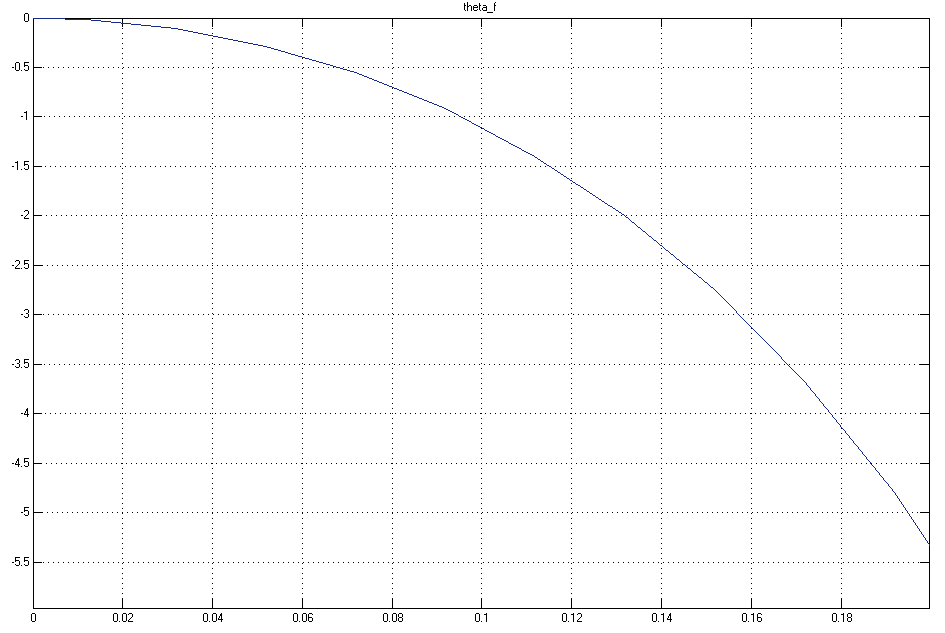
\includegraphics[scale=0.5]{figures/stepResponseBlocks}
	\centering
	\captionsetup{justification=centering}	
	\caption{Step response of the system from \figref{systemSimulink}}
	\label{stepCubliBlocks}
\end{figure}